\documentclass[]{article}
\usepackage{graphicx}
\usepackage{subcaption}
\graphicspath{{images/}}

%opening
\title{RL e09}
\author{Mengnan Wang}

\begin{document}

\maketitle

\section{SMDP learning in four-room domain}
\subsection{Computing policies for options}
\paragraph{}I only compute 4 policy for moving to up/left/right/down door.
These policies can be used in any one of four rooms with correct coordinate mapping.
\begin{figure}
	\centering
	\begin{subfigure}[b]{0.475\textwidth}
		\centering
		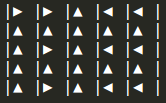
\includegraphics[width=.9\linewidth]{up_policy.png}
		\caption{Up-door policy}
	\end{subfigure}
	\begin{subfigure}[b]{0.475\textwidth}
		\centering
		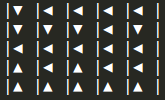
\includegraphics[width=.9\linewidth]{left_policy.png}
		\caption{Left-door policy}
	\end{subfigure}
	\begin{subfigure}[b]{0.475\textwidth}
		\centering
		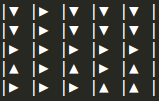
\includegraphics[width=.9\linewidth]{right_policy.png}
		\caption{Right-door policy}
	\end{subfigure}
	\begin{subfigure}[b]{0.475\textwidth}
		\centering
		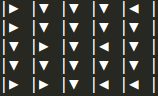
\includegraphics[width=.9\linewidth]{down_policy.png}
		\caption{Down-door policy}
	\end{subfigure}
	\caption{Option policy}
\end{figure}

\subsection{SMDP planning}
\paragraph{}'U' stands for moving to up door. 'L' stands for moving to left door. 'D' stands for moving to down door. 'R' stands for moving to right door.
\paragraph{}Compared to basic Q-Learning without options. SMDP explores less states, which can be seen in Q value plot. Update type 1 explores less than naive update. But for update type 2, it does not converge after 1000 iteration. As i increase the iteration, it converges at 10000 iteration and the final policy and value plot is similar to basic Q-Learning without options.
\begin{figure}
	\centering
	\begin{subfigure}[b]{0.475\textwidth}
	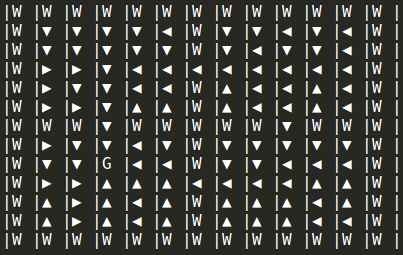
\includegraphics[width=\linewidth]{basic_q.png}
	\caption{Policy of Q-Learning}
	\end{subfigure}
	\begin{subfigure}[b]{0.475\textwidth}
		\centering
		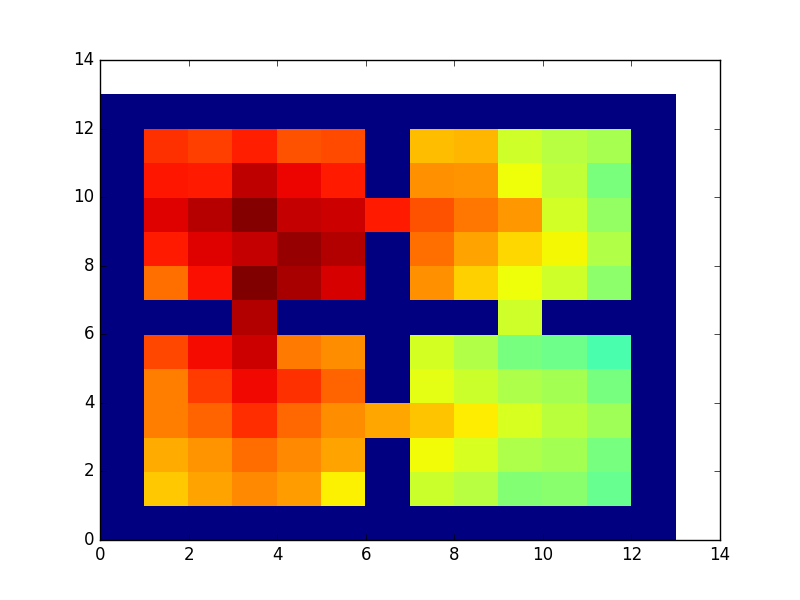
\includegraphics[width=.9\linewidth]{basic_q_value_plot.png}
		\caption{Q value of Q-Learning}
	\end{subfigure}
	\caption{Basic Q-Learning with 1000 iterations}
\end{figure}

\begin{figure}
	\centering
	\begin{subfigure}[b]{0.475\textwidth}
		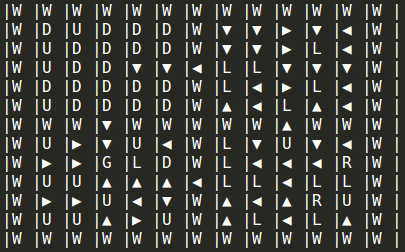
\includegraphics[width=\linewidth]{naive_update_policy.png}
		\caption{Policy of Q-Learning}
	\end{subfigure}
	\begin{subfigure}[b]{0.475\textwidth}
		\centering
		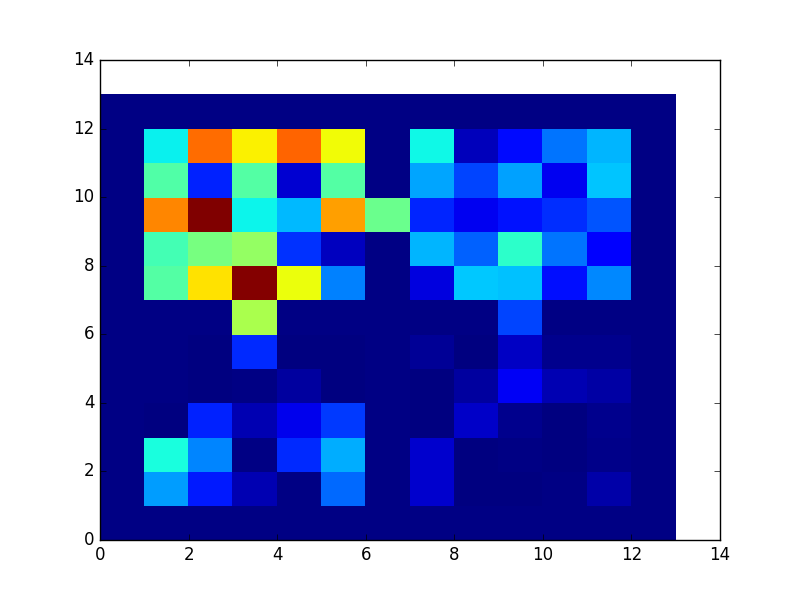
\includegraphics[width=.9\linewidth]{naive_update_value_plot.png}
		\caption{Q value of Q-Learning}
	\end{subfigure}
	\caption{SMDP with naive update after 1000 iterations}
\end{figure}

\begin{figure}
	\centering
	\begin{subfigure}[b]{0.475\textwidth}
		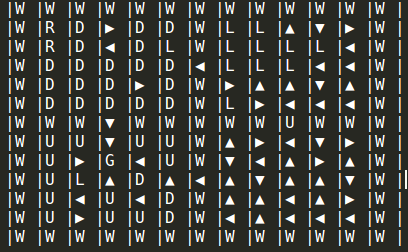
\includegraphics[width=\linewidth]{update_1_policy.png}
		\caption{Policy of Q-Learning}
	\end{subfigure}
	\begin{subfigure}[b]{0.475\textwidth}
		\centering
		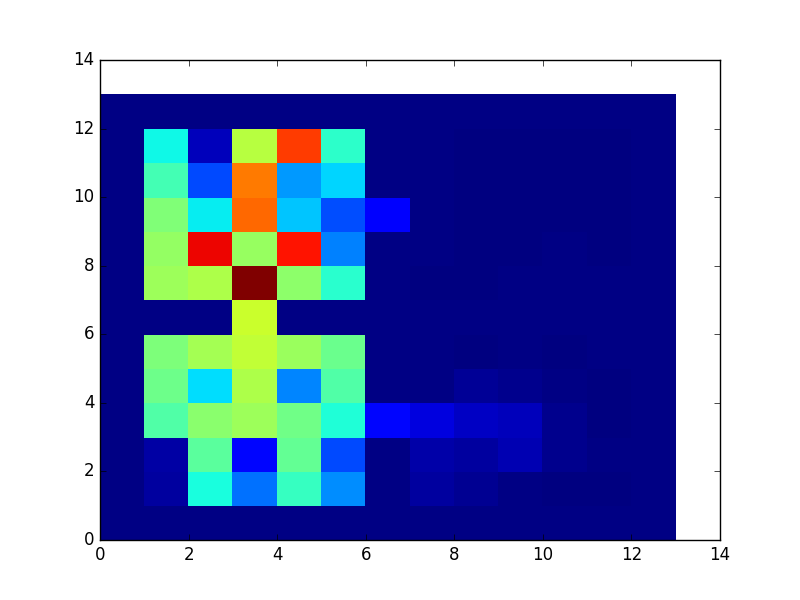
\includegraphics[width=.9\linewidth]{update_1_value_plot.png}
		\caption{Q value of Q-Learning}
	\end{subfigure}
	\caption{SMDP with update type 1 after 1000 iterations}
\end{figure}

\begin{figure}
	\centering
	\begin{subfigure}[b]{0.475\textwidth}
		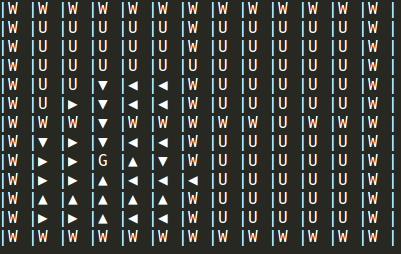
\includegraphics[width=\linewidth]{update_2_policy.png}
		\caption{Policy of Q-Learning}
	\end{subfigure}
	\begin{subfigure}[b]{0.475\textwidth}
		\centering
		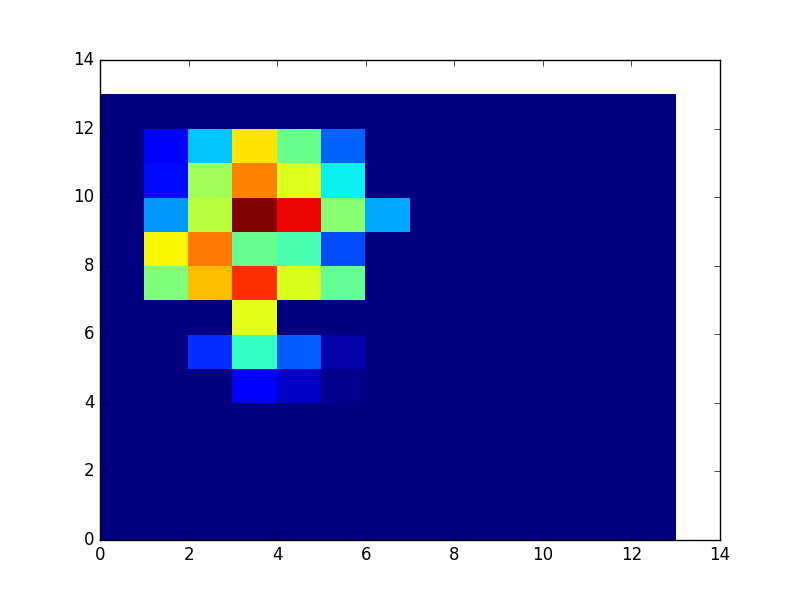
\includegraphics[width=.9\linewidth]{update_2_value_plot.png}
		\caption{Q value of Q-Learning}
	\end{subfigure}
	\caption{SMDP with update type 2 after 1000 iterations}
\end{figure}

\begin{figure}
	\centering
	\begin{subfigure}[b]{0.475\textwidth}
		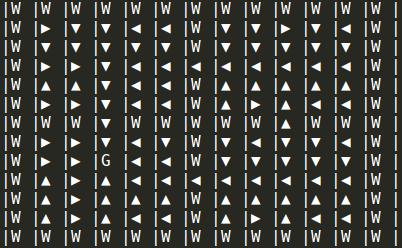
\includegraphics[width=\linewidth]{update_2_policy2.png}
		\caption{Policy of Q-Learning}
	\end{subfigure}
	\begin{subfigure}[b]{0.475\textwidth}
		\centering
		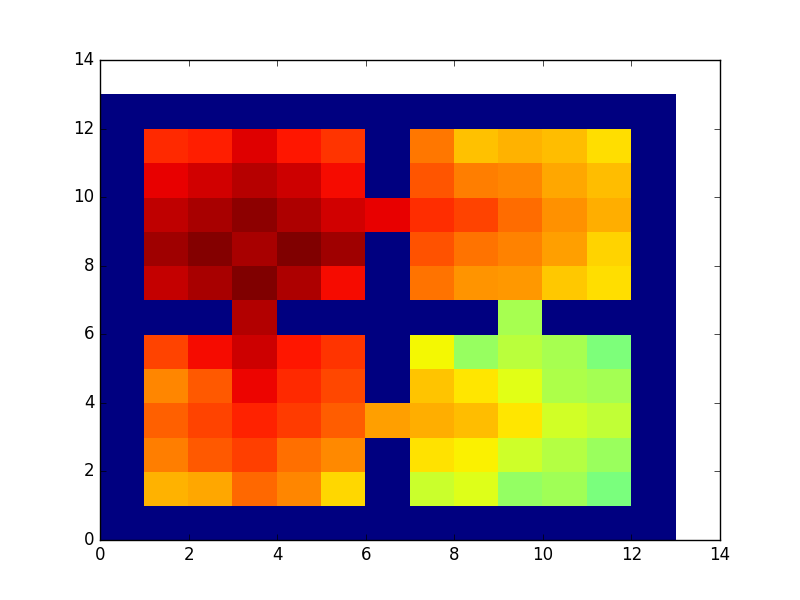
\includegraphics[width=.9\linewidth]{update_2_value_plot2.png}
		\caption{Q value of Q-Learning}
	\end{subfigure}
	\caption{SMDP with pdate type 2 after 10000 iterations}
\end{figure}

\subsection{Compute P}
\paragraph{}To estimate $P(s^{'},k|s,o)$, we can record the transition $\{s,o,r,s^{'},k\}$ and compute the expectation.

\end{document}
